% ****** Start of file apssamp.tex ******
%
%   This file is part of the APS files in the REVTeX 4.1 distribution.
%   Version 4.1r of REVTeX, August 2010
%
%   Copyright (c) 2009, 2010 The American Physical Society.
%
%   See the REVTeX 4 README file for restrictions and more information.
%
% TeX'ing this file requires that you have AMS-LaTeX 2.0 installed
% as well as the rest of the prerequisites for REVTeX 4.1
%
% See the REVTeX 4 README file
% It also requires running BibTeX. The commands are as follows:
%
%  1)  latex apssamp.tex
%  2)  bibtex apssamp
%  3)  latex apssamp.tex
%  4)  latex apssamp.tex
%
\documentclass[
 reprint,
%superscriptaddress,
%groupedaddress,
%unsortedaddress,
%runinaddress,
%frontmatterverbose, 
%preprint,
showpacs,
%preprintnumbers,
%nofootinbib,
%nobibnotes,
%bibnotes,
 amsmath,amssymb,
 aps,
pra,
%prb,
%rmp,
%prstab,
%prstper,
%floatfix,
]{revtex4-1}

\usepackage{graphicx}% Include figure files
\usepackage{dcolumn}% Align table columns on decimal point
\usepackage{bm}% bold math
%\usepackage{hyperref}% add hypertext capabilities
%\usepackage[mathlines]{lineno}% Enable numbering of text and display math
%\linenumbers\relax % Commence numbering lines

%\usepackage[showframe,%Uncomment any one of the following lines to test 
%%scale=0.7, marginratio={1:1, 2:3}, ignoreall,% default settings
%%text={7in,10in},centering,
%%margin=1.5in,
%%total={6.5in,8.75in}, top=1.2in, left=0.9in, includefoot,
%%height=10in,a5paper,hmargin={3cm,0.8in},
%]{geometry}


\def\v#1{{\bf#1}}
\def\be{\begin{equation}}
\def\ee{\end{equation}}
\def\bea{\begin{eqnarray}}
\def\eea{\end{eqnarray}}
\def\ahalf{{\textstyle{1\over2}}}
\def\twet{{\textstyle{2\over3}}}
\newcommand{\bfalpha}{\mbox{\boldmath$\alpha$\unboldmath}}
\newcommand{\bfbeta}{\mbox{\boldmath$\beta$\unboldmath}}
\newcommand{\bfxi}{\mbox{\boldmath$\xi$\unboldmath}}
\newcommand{\bfeta}{\mbox{\boldmath$\eta$\unboldmath}}
\newcommand{\bfsigma}{\mbox{\boldmath$\sigma$\unboldmath}}
\newcommand{\bfpi}{\mbox{\boldmath$\pi$\unboldmath}}
\newcommand{\bfgamma}{\mbox{\boldmath$\gamma$\unboldmath}}
\newcommand{\bfrho}{\mbox{\boldmath$\rho$\unboldmath}}
\newcommand{\bfkappa}{\mbox{\boldmath$\kappa$\unboldmath}}
\newcommand{\sg}{\mbox{\rm sg}}
\def\ie{{\it i.e.\,}}
\def\etal{{\it et al.   }}
\def\ocal{\mbox{$\cal O\,$}}
\def\ycal{\mbox{$\cal Y\,$}}
\def\lcal{\mbox{$\cal L\,$}}
\def\ecal{\mbox{$\cal E\,$}}
\def\hcal{\mbox{$\cal H\,$}}
\def\ncal{\mbox{$\cal N\,$}}
\def\<{\langle}
\def\>{\rangle}



\begin{document}

%\preprint{APS/123-QED}

\title{Transparent lattices and their solitary waves}% Force line breaks with \\
%\thanks{A footnote to the article title}%

\author{E. Sadurn\'i}
 \email{sadurni@ifuap.buap.mx}
\affiliation{Instituto de F\'isica, Benem\'erita Universidad Aut\'onoma de Puebla,
Apartado Postal J-48, 72570 Puebla, M\'exico}


\date{\today}% It is always \today, today,
             %  but any date may be explicitly specified

\begin{abstract}
Transparent tight-binding arrays are discussed through a generalization of supersymmetric quantum mechanics in discrete variables. A finite-difference Darboux transformation is applied to the scattering matrix of a periodic array, rendering reflectionless systems with non-trivial potentials and site-dependent hopping parameters. A procedure for constructing a hierarchy of discrete hamiltonians is indicated and a particular biparametric family is given. The corresponding potentials and hopping functions are identified as solitary waves, pointing to a discrete spinorial generalization of the Korteweg-deVries family. 
\end{abstract}

\pacs{42.50.Md, 42.81.Dp, 04.60.Nc, 11.30.Pb}

%\keywords{Suggested keywords}

\maketitle

%\tableofcontents

\section{ Introduction \label{sec:1}}

There is an increasing interest in the study of tight-binding models and their application to several areas, such as optical waveguides \cite{russell2003, keil2010, foresi1997}, ultracold atoms in optical lattices \cite{oberthaler2006, bloch2005, oberthaler1996} and artificial realizations of condensed matter, e.g. graphene \cite{esslinger2013, kuhl2010, barkhofen2013, bittner2010, bellec2013}. The subject has reached the domain of supersymmetric models through a recent realization of a Dirac oscillator \cite{franco2013, sadurni2010, longhi2010}, which seems to be the first experimental construction of an $N=2$ supersymmetry. In these applications, technical developments towards the engineering of local potentials and couplings between sites have been reached with several purposes \cite{esslinger2008, christodoulides2008}, even with microwaves \cite{sadurni2013}. A particular example of interest is the perfect transmission of signals through discrete arrays and its associated scattering problem in the presence of local lattice modifications. It is important to mention that transparency has been extensively studied in continuous variables \cite{cooper1995, samsonov2000}, but never in a tight-binding array \cite{berry2008}. In this paper we provide an elegant solution of the problem by extending the well-developed apparatus of supersymmetric quantum mechanics \cite{kac1973, catterall2002} (SUSYQM) to discrete variables. 

We shall proceed in the following order: In section \ref{sec:2} we define our problem and state the main result of our work by giving a family of transparent potentials in tight-binding arrays. Section \ref{sec:3} provides the necessary definitions and generalizations for discrete SUSYQM. This section can be read separately and is divided in three parts: \ref{sec:3.0} The factorization method, \ref{sec:3.1} isospectrality and transparency (where we address the problem of discrete-variable Darboux transformations) and \ref{sec:3.2} the continuous limit. Section \ref{sec:4} provides a numerical check of the required properties. In full analogy with traditional SUSYQM, section \ref{sec:4} studies a family of models which constitute a set of discrete solitons given by potentials and hopping parameters.  Section \ref{sec:5} gives a brief conclusion. 

\section{A family of models \label{sec:2}}

\begin{figure}[t]
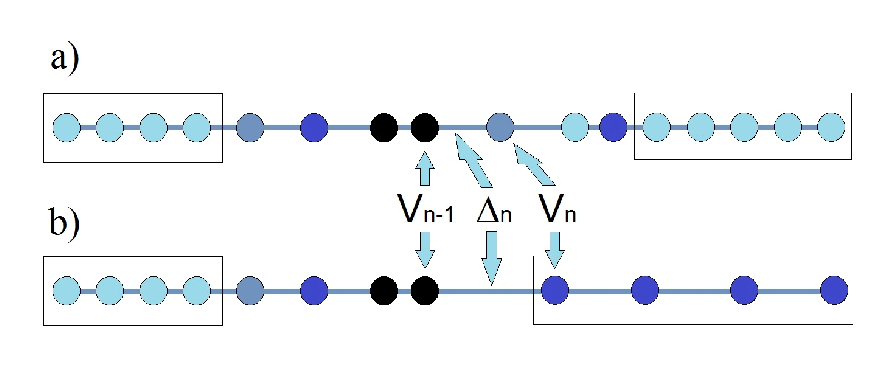
\includegraphics[width=8.6cm]{twochains} 
\caption{\label{fig:0} Two asymptotically periodic arrays. Bonds represent couplings $\Delta_n$ and site colors represent potential values $V_n$. Example a) has two identical asymptotic regions indicated by rectangular boxes. In example b), the asymptotically periodic regions do not coincide.}
\end{figure}

Several areas benefit from second quantized tight-binding models with and without particle interactions. In one dimension, one typically has

\bea
H_{\mbox{\small quantum}} = \sum_{\< n, m\>} \left[\Delta_{nm} C^{\dagger}_n C_m +  \Delta_{nm}^*  C^{\dagger}_m C_n  \right]
\label{a1}
\eea
%
where $C_n, C_m^{\dagger}$ are local field operators of bosonic or fermionic nature. The off-diagonal $\Delta_{nm}$'s are hopping parameters and the diagonal $\Delta_{nn}$ represent on-site potentials. The propagation of signals in such models can be viewed as a scattering problem in which one or many particle states with well defined momenta can be ideally prapared at infinity. In the absence of terms of the form $C_n^{\dagger} C_m C_i^{\dagger} C_j$ (dilute matter waves \cite{zoller1998} or photonic crystal waveguides \cite{chien2007}), the lack of particle interactions allow a single-particle treatment of the scattering problem. Therefore, we restrict ourselves to a hamiltonian in first quantization. With the help of Wannier functions $\< x | n \>$ localized around site $n$, we have

\bea
H = \sum_{n} \Delta_n | n \>\<n-1| + \Delta_n^* | n-1 \>\<n| + V_n | n \>\<n|.
\label{a2}
\eea 
%
For simplicity, only nearest neighbors are assumed. One can expand a stationary state $|\psi \>$ as

\bea
|\psi \> = \sum_{n} \psi_n | n \>
\label{a3}
\eea
%
and from this expansion, the Schr\"odinger equation associated to (\ref{a2}) acquires its typical recurrence form

\bea
\Delta_n \psi_{n-1} + \Delta_{n+1} \psi_{n+1} + V_n \psi_n = E \psi_n.
\label{a4}
\eea
%
Now we define $H$ to be {\it asymptotically periodic\ }if at the far ends of the array (left and right) we have asymptotically constant couplings and potentials, i.e. $\Delta_{n} \sim \Delta_0$ and $V_n \sim V_0$  if $n >> 1$ . A diagram is shown in figure \ref{fig:0}. The main finding of this work is the existence of a family of potentials and hopping paramaters (or functions, since they depend on site $n$) for which the reflection coefficient of a Bloch wave vanishes for all energies. The most general expression for the biparametric family can be written in terms of continued fractions, as we shall see in section \ref{sec:5}. To this end, we employ the notation

\bea
\left[a_n, b_n; a_{n-1}, b_{n-1}; ... \right] = a_n + \frac{b_n}{a_{n-1} + \frac{b_{n-1}}{\cdots}}.
\label{a6}
\eea
%
An important case is given by a monoparametric subfamily $\tilde V_n, \tilde \Delta_n$, which can be written in terms of hyperbolic functions

\bea
\tilde V_n = V_0  + \Delta_0\left(\frac{\cosh\left[ n \lambda + \beta \right]}{\cosh\left[ (n-1) \lambda + \beta \right]} - \frac{\cosh\left[ (n+1) \lambda + \beta \right]}{\cosh\left[ n \lambda + \beta \right]}\right), \nonumber \\ 
\label{a7}
\eea
%
\bea
\tilde \Delta_n = \Delta_0 \frac{\sqrt{ \cosh \left[ (n-2) \lambda + \beta \right] \cosh \left[ n \lambda + \beta \right] } }{ \cosh \left[ (n-1) \lambda + \beta \right] },\nonumber \\ 
\label{a8}
\eea
%
where $\beta$ is a free parameter and the convenient definition 
\bea
\lambda = \ahalf \ln \left(\frac{V_0-\sqrt{V_0^2 - 4 \Delta_0^2}}{V_0+\sqrt{V_0^2 - 4 \Delta_0^2}}\right) 
\label{a9}
\eea
%
has been used. Some examples are depicted in figure \ref{fig:1} as a function of $\gamma=\mbox{e}^{2\beta}$. In the following section we give a detailed method of derivation with the help of discrete SUSYQM.

\begin{figure*}[t]
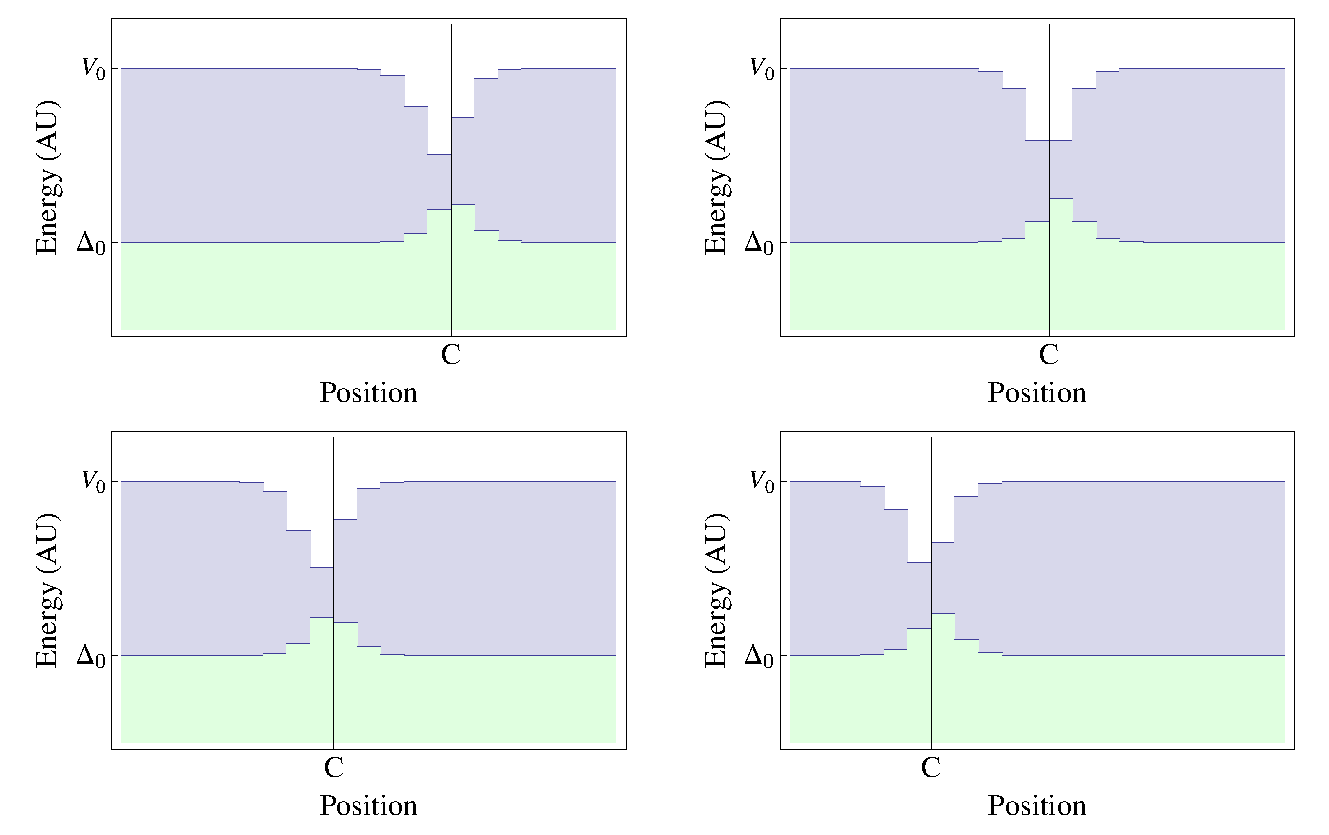
\includegraphics[width=10.6cm]{fig1}
%\begin{tabular}{ll} \includegraphics[width=5.3cm]{potential24} & \includegraphics[width=5.3cm]{potential23} \\ \includegraphics[width=5.3cm]{potential22} & %\includegraphics[width=5.3cm]{potential21} \end{tabular} 
\caption{\label{fig:1} Variation of our discrete potential (blue-filled curve) and hopping function (green-filled curve) with respecto to $\gamma$. The minimum of the potential and the maximum of the hopping parameter lie in the same region and suffer a linear displacement to the right when $\gamma$ is increased exponentially (the center is denoted by C).}
\end{figure*}


\section{A path to discrete SUSYQM \label{sec:3}}
\subsection{The discrete factorization method \label{sec:3.0}}
 The central discretization of the Schr\"odinger equation leads naturally to a nearest-neighbor tight-binding hamiltonian, therefore we focus on such local quantum-mechanical models for our constructions. A generic expression for $H$ in terms of operators can be written as

\bea
H = \Delta(N) T + T^{\dagger} \Delta(N)^{\dagger} + V(N),
\label{e1}
\eea
%
where $N$ is the site number operator and $T$ is a translation in one unit. These operators satisfy $\left[ F(N), T \right]= T \{F(N+1)-F(N) \}$ for any function $F$. Their action on localized states $|n\>$ is given by $N|n\> = n |n\>$ and $T |n\> = |n+1\>$. The functions $V(N)$ and $\Delta(N)$ represent the on-site potential and the nearest- neighbor hopping function, respectively. Their eigenvalues are $V_n$ and $\Delta_n$, with $V_n$ real. In full analogy with traditional SUSYQM in continuous variables, we propose a factorization scheme of (\ref{e1}) as follows 

\bea
H = A^{\dagger} A, \quad A =  F(N)T + G(N).
\label{e2}
\eea
%
The reconstruction of (\ref{e1}) will be possible if we impose the restrictions $V_n = |G_n|^2 + |F_{n+1}|^2$ and $\Delta_n = G_{n}^* F_n$, as can be verified by applying the product $A^{\dagger} A$ to some state $|n\>$. It is important to recognize that this scheme can be applied only if the potential is positive definite or, without loss of generality, if it is bounded below. This property enables us to consider the existence of a ground state and to further subtract it from the hamiltonian, which is a usual procedure \cite{cooper1995}. We should also point out that given a positive $V_n$ and a complex $\Delta_n$, we may determine $F_n$ and $G_n$ up to phase factors (which can be gauged away trivially in 1D). To this end one has to solve the recurrence $V_n = |F_{n+1}|^2 + |\Delta_n|^2 / |F_n|^2$ for $|F_n|^2$ by the method of continued fractions

\bea
|F_n|^2 = \left[ V_{n-1}, |\Delta_{n-1}|^2;V_{n-2}, |\Delta_{n-2}|^2;... \right]
\label{e3}
\eea
%
and then reconstruct $G$ with the relation

\bea
|G_n|^2 = \frac{|\Delta_n|^2}{\left[ V_{n-1}, |\Delta_{n-1}|^2;V_{n-2}, |\Delta_{n-2}|^2;... \right]}.
\label{e4}
\eea
%

Our proposal for the factorization of $H$ is in full correspondence with the continuous case, in view of the analogy $ A_{\mbox{\small discrete}} \leftrightarrow  A_{\mbox{\small continuous}}$, i.e.

\bea
F(N) T + G(N) \longleftrightarrow \frac{d}{dx} + W(x),
\label{e4}
\eea
%
where $W(x)$ is a superpotential satisfying the Riccati equation \cite{cooper1995}. A clear connection with continuous variables can be given by means of a lattice spacing $a$: The translation of wave functions $\<x-a|n\>=\<x|n+1\>$ motivates the substitutions $T=\exp (- a \cdot d/dx),  x= aN$, which in turn lead to the limit   

\bea
F \left(\frac{x}{a} \right)\exp \left(- a \frac{d}{dx} \right) + G \left(\frac{x}{a} \right) \longrightarrow \phi(x) \frac{d}{dx} + \gamma(x).\nonumber \\
\label{e5}
\eea
%
Here we have imposed $F(x/a) + G(x/a) \rightarrow \gamma(x)$ and $aF(x/a) \rightarrow -\phi(x)$. This limit resembles the usual Darboux operator \cite{darboux1882, manas1997}. Moreover, our discrete $A$ in (\ref{e2}) is a particular case of a series of automorphisms, but we should stress that  $F(N) \neq \mbox{constant}$ is a more general choice and allows more freedom in our models. In connection with singularities in our limits, we should note that $a F(x/a)$ is regular at $a=0$, but $F(x/a)$ is not. The function $G(x/a)$ compensates for the singularity of $F(x/a)$ rendering a finite $\gamma(x)$. We shall come back to this point in connection with the P\"oschl-Teller potential as a plausible continuous limit.

With these considerations, we are ready to construct a discrete superpartner $\tilde H$ with the prescription

\bea
\tilde H = AA^{\dagger}= \tilde \Delta(N) T +  T^{\dagger} \tilde \Delta(N)^{\dagger} + \tilde V(N).
\label{e6}
\eea
%
The new potential and hopping functions are given by

\bea
\tilde \Delta(N) = G(N-1)^{\dagger} F(N), 
\label{e7}
\eea
%
\bea
\tilde V(N) =   G(N)G(N)^{\dagger} + F(N)F(N)^{\dagger},
\label{e8}
\eea
%
and their eigenvalues obey the relations $\tilde \Delta_n = G_{n-1}^* F_{n}, \tilde V_n = |G_{n}|^2 + | F_{n}|^2$. Remarkably, the functions which determine the superpartners come in pairs, since both $\Delta$ and $V$ must be modified.

\subsection{Isospectrality and Transparency \label{sec:3.1} }

Our method can be readily applied to bound states as well as scattering solutions. Let $|\psi_k\>$ be a solution of $H|\psi_k\>=E_k|\psi_k\>$. If $\tilde H|\tilde \psi_k\>= \tilde E_k| \tilde \psi_k\>$, we deduce the relations

\bea
|\tilde \psi_{k} \> = \left( E_{k+1} - E_0 \right)^{-1/2} \{ F(N)T + G(N) \} |\psi_{k+1} \>, \nonumber \\
\label{e9}
\eea
%
\bea
\tilde E_{k} = E_{k+1}.
\label{e10}
\eea
%
The $N=2$ supersymmetry is realized by defining supercharges with the help of $A, A^{\dagger}$ and the Pauli matrices $\sigma_{\pm}$. We have 

\bea
Q=\sigma_- A, \quad Q^{\dagger}=\sigma_+ A^{\dagger}, \quad \hcal = \{ Q, Q^{\dagger} \}. 
\label{e10.1}
\eea
%
where $\hcal$ is the central charge. The aforementioned isospectrality can be used for many purposes, but we are interested now in the transformation properties of the scattering matrix and their relation with transparency.

Let us define the conditions of a scattering problem in discrete variables. We take $H, \tilde H$ asymptotically periodic, such that in the limit $n \rightarrow \pm \infty$ we have $V_n \rightarrow V_{\pm}, \tilde V_n \rightarrow \tilde V_{\pm}, \Delta_n \rightarrow \Delta_{\pm}, \tilde \Delta_n \rightarrow \tilde \Delta_{\pm}$. The solutions with continuous parameter $k$ become Bloch waves: $\< n| \psi_k\> \rightarrow \ncal \mbox{e}^{ikn} $ and similarly for $\< n| \tilde \psi_k\>$. The limit values of $F$ and $G$ can be reconstructed via the relations $|F_{\pm}|^2= \ahalf (V_{\pm} \pm \sqrt{V_{\pm}^2-4\Delta_{\pm}^2})$, where $V_{\pm}^2 \geq 4 \Delta_{\pm}^2$. With this information on the factorization parameters, we are ready to apply the discrete Darboux transformation to the asymptotic form of the wave functions

\bea
\< n |A| \psi_k \> = \left( G_n + \mbox{e}^{ik} F_n \right) \psi_n^{k} \rightarrow  \left( G_{\pm} + \mbox{e}^{ik} F_{\pm} \right) \mbox{e}^{ikn}. \nonumber \\
\label{e11}
\eea
%
It may happen that the asymptotic regions at $\pm \infty$ have different associated constants, i.e. $V_+ \neq V_-, \Delta_+ \neq \Delta_-$. However, we always have the energy (or dispersion) relation $E = 2 \Delta_- \cos k + V_- = 2 \Delta_+ \cos k' + V_+$ satisfied at both ends of the array. In general $k'\neq k$, and the reflected and transmitted waves have different Bloch quasi-momenta, expressed by the limits

\bea
\<n | \psi_k \> \begin{array}{c} _{\longrightarrow} \\  _{n \rightarrow -\infty} \end{array} \mbox{e}^{ikn} + R \mbox{e}^{-ikn},
\label{e12}
\eea
%
\bea
\<n | \psi_k \> \begin{array}{c} _{\longrightarrow} \\  _{n \rightarrow +\infty} \end{array}  T \mbox{e}^{ik'n}.
\label{e13}
\eea
%
The application of the discrete Darboux transformation (\ref{e11}) to (\ref{e12}) and (\ref{e13}) leads to waves of the same energy but with modified transmission and reflection coefficients $\tilde T, \tilde R$. The results are

\bea
\tilde R = \left( \frac{G_- + \mbox{e}^{ik}F_-}{G_- + \mbox{e}^{-ik}F_-} \right) R
\label{e14}
\eea
%
\bea
\tilde T = \left( \frac{G_+ + \mbox{e}^{ik'}F_+}{G_- + \mbox{e}^{-ik}F_-} \right) T
\label{e15}
\eea
%
which constitute a generalization of the usual scattering matrix transformations with the replacement $ik \mapsto e^{ik}$. The reality condition for $G_{-}$ and  $F_-$ establishes that $|\tilde R|= |R|$. Moreover, in the problem of transparency $\tilde R$ vanishes if $R=0$.  Let us examine this possibility by proposing $H$ as a {\it free\ }hamiltonian, i.e. a periodic chain. This means that $\Delta_n=\Delta_{\pm} \equiv \Delta_0$ and $V_n=V_{\pm} \equiv V_0$. Now we must find $\tilde V_n$ and $\tilde \Delta_n$ by solving the recurrence 

\bea
|G_n|^2 = V_0 - |F_{n+1}|^2 = \frac{|\Delta_0|^2}{ |F_{n}|^2}
\eea 
%
for $|F_n|^2$. With the definitions $\mu_{\pm} = \ahalf (V_{0} \pm \sqrt{V_{0}^2-4\Delta_{0}^2})$ we obtain

\bea
F_n = \sqrt{\frac{\alpha_+ \mu_+ ^{n} + \alpha_- \mu_- ^{n}}{\alpha_+ \mu_+ ^{n-1} + \alpha_- \mu_- ^{n-1}}},  
\label{e16}
\eea
%
\bea
G_n = \Delta_0 \sqrt{\frac{\alpha_+ \mu_+ ^{n-1} + \alpha_- \mu_- ^{n-1}}{\alpha_+ \mu_+ ^{n} + \alpha_- \mu_- ^{n}}}, 
\label{e17}
\eea
%
where $\alpha_{\pm}$ are arbitrary constants of the same sign, preserving the reality of $F_n$. The potential and hopping functions are now

\bea
\tilde V_n = V_0  + \frac{\alpha_+ \mu_+ ^{n} + \alpha_- \mu_- ^{n}}{\alpha_+ \mu_+ ^{n-1} + \alpha_- \mu_- ^{n-1}} - \frac{\alpha_+ \mu_+ ^{n+1} + \alpha_- \mu_- ^{n+1}}{\alpha_+ \mu_+ ^{n} + \alpha_- \mu_- ^{n}} \nonumber \\ 
\label{e18}
\eea
%
\bea
\tilde \Delta_n = \Delta_0 \frac{\sqrt{ (\alpha_+ \mu_+ ^{n} + \alpha_- \mu_- ^{n})(\alpha_+ \mu_+ ^{n-2} + \alpha_- \mu_- ^{n-2}) } }{ \alpha_+ \mu_+ ^{n-1} + \alpha_- \mu_- ^{n-1} }.\nonumber \\ 
\label{e19}
\eea
%
Finally, $\tilde H$ given in (\ref{e6}) is a non-trivial monoparametric familiy enjoying the property of being reflectionless. One can show that the solutions depend only on $\gamma \equiv \alpha_- / \alpha_+$, and that $\tilde V, \tilde \Delta$ can be put in terms of hyperbolic functions $\sinh ( n \ln \mu_{\pm}), \cosh ( n \ln \mu_{\pm})$. In figure \ref{fig:1} we show the behavior of potentials and hopping parameters under the modification of $\gamma$, resulting in a translation of the interaction region or potential well. This is reminiscent of shape invariance in continuous variables, where generalized P\"oschl-Teller or Scarf potentials can be translated at will on the real line (among other operations, such as rescaling). However, such a similarity is to be taken with a grain of salt, since continuous translations of discrete variables yield the same (translated) potentials only if $\nu = \ln(\gamma) / \ln (\mu_+ / \mu_-)$ is an integer. We can distinguish these features in the panels of figure \ref{fig:1}, as the centers of $\tilde V, \tilde \Delta$ move to the right and the functions suffer slight variations for non-integer values of $\nu$.

\begin{figure*}[t]
\includegraphics[width=10.6cm]{fig2}
%\begin{tabular}{ll} \includegraphics[width=5.3cm]{wave2766} & \includegraphics[width=5.3cm]{wave2780} \\ \includegraphics[width=5.3cm]{wave2791} & \includegraphics[width=5.3cm]%{wave2797} \end{tabular} 
\caption{\label{fig:2} Numerical solutions of the scattering problem in discrete variable $n$ for a Bloch wave impinging from the left. Each panel shows a different scattering energy $E$. The parameters are $\gamma=\mbox{e}^{-6}$, $V_0 = 6 \Delta_0$. Solid gold: $|\tilde \psi|$, dashed blue:  $\mbox{Re}(\tilde \psi)$,  dashed red:  $\mbox{Im}(\tilde \psi)$, blue-filled curve: $\tilde V$, red-filled curve: $\tilde \Delta$, solid black: $E$. In all cases $|T|^2 = 1$ and the original Bloch wave picks up a phase at the right end of the array.}
\end{figure*}


\subsection{The continuous limit \label{sec:3.2}}

It is important to make contact with the well-known results of transparent potentials in continuous SUSYQM. The limits can be reached by letting $a \rightarrow 0$ as before. In order to recover a Schr\"odinger equation with double derivatives and ground state energy $U_0$, we must impose $x=an$, $\Delta_0 \sim - R_0 / a^2$ with $R_0 >0$ and $V_0 + 2\Delta_0 \sim U_0$. In the process, we note that $T \sim 1 - a\cdot d/dx$ and $(\mu_+ / \mu_-)^n \sim \exp \left(4x\sqrt{R_0/U_0} \right)$. The particular choice $\gamma=1$ leads to a familiar case of hyperbolic superpotentials; we have

\bea
F_n \sim \frac{\sqrt{R_0}}{a} + \sqrt{\frac{U_0}{R_0}} \tanh \left( 2\sqrt{\frac{U_0}{R_0}} x \right),
\label{e21}
\eea
%
\bea
G_n \sim -\frac{\sqrt{R_0}}{a} + \sqrt{\frac{U_0}{R_0}} \tanh \left( 2\sqrt{\frac{U_0}{R_0}} x \right),
\label{e22}
\eea
%
and the Darboux operator becomes

\bea
A \sim 2\sqrt{\frac{U_0}{R_0}} \tanh \left( 2\sqrt{\frac{U_0}{R_0}} x \right) + \sqrt{R_0} \frac{d}{dx}.
\label{e23}
\eea
%
This is the usual operator for the Rosen-Morse superpotential with non-zero ground state $U_0$.



\section{A numerical test for transparency \label{sec:4}}
We test the reflectionless property by solving numerically the scattering problem for various energies. A reasonable choice of parameters for the potential and hopping functions is $\gamma=e^{-6}$ (producing strong asymmetry in the potential) and $V_0/\Delta_0 = 6$, localizing the region of interaction in a small portion of a few sites. The numerical solution is reached by imposing a Bloch wave at least at two sites, since (\ref{a4}) is a second order recurrence. For instance, at sites $n=0$ and $n=1$ we have

\bea
\tilde \psi_0 = \mbox{e}^{i \times 0}= 1,\quad \tilde \psi_1 = \mbox{e}^{ik}.
\eea
%
Such boundary conditions generate $\tilde \psi_{n+1}$ through the recurrence
\bea
\tilde \psi_{n+1} = \frac{ \tilde \Delta_n \tilde \psi_{n-1} +  (E-\tilde V_n)\tilde \psi_n}{\tilde \Delta_{n+1}},
\label{e20}
\eea
%
provided that $E$ and $k$ are related by $E=V_0 + \Delta_0 \cos k$. We have used four different energies in the scattering regime: $E/\Delta_0 = 7.66, 7.80, 7.91, 7.97$, verifying that the modulus of the {\it transmitted\ }wavefunction recovers the value $1$ in all cases. The results are shown in figure \ref{fig:2}, where the modulus, the real and the imaginary part of $\psi_n$ are displayed. At the right end of the array (25 sites) the wave recovers its modulus and phase factor, but at this region the potential is negligible and the solution will continue to be a Bloch wave propagating to the right if the array is prolonged indefinitely.

\begin{figure*}[t]
\includegraphics[width=10.6cm]{fig3}
%\begin{tabular}{ll} \includegraphics[width=5.3cm]{discretesolitons21} & \includegraphics[width=5.3cm]{discretesolitons22} \\ \includegraphics[width=5.3cm]{discretesolitons23} & %\includegraphics[width=5.3cm]{discretesolitons24} \end{tabular}
\caption{\label{fig:3} The motion of discrete solitonic potentials (blue-filled curve) and solitonic hopping functions (green-filled curve). The parameter $\alpha = 1.5$ produces two solitons (a maximum and a minimum) for each graph. As $\gamma$ increases, their centers $C_1$ and $C_2$ move to the right at different velocities. This is shown progressively from top left to right bottom.}
\end{figure*}

\section{Biparametric solitons \label{sec:5}}

The solutions of the Korteweg-deVries (KdV) equation \cite{kruskal1967, kdv1895} are known to be represented by a hierarchy of superpotentials \cite{wang1990}. Such a hierarchy can be obtained through a step-by-step method for generating superpartners. In our discrete case, however, the application of new Darboux transformations can be increasingly challenging. Yet, a simpler strategy to obtain families of solutions consists of finding at once all the superpartners of a given reflectionless problem. We proceed in this direction in what follows. Let us start with a monoparametric transparent problem given by (\ref{e18}) and (\ref{e19}). We now consider a hamiltonian

\bea
H^{(\alpha)} = \Delta^{(\alpha)}(N) T + T^{\dagger} \Delta^{(\alpha)}(N)^{\dagger} + V^{(\alpha)}(N),
\label{e24}
\eea
%
where $\alpha$ is a new parameter, yet to be determined. The factorization procedure yields the relations

\bea
V^{(\alpha)}_n = |G_n^{(\alpha)}|^2 + |F_{n+1}^{(\alpha)}|^2, \nonumber \\ \Delta^{(\alpha)}_n = \left[G_n^{(\alpha)}\right]^* F_n^{(\alpha)},
\label{e25}
\eea
%
but another set of recurrences in terms of $\tilde V_n$ and $\tilde \Delta_n$ must be satisfied for the reflectionless problem:
\bea
\tilde V_n = |G_n^{(\alpha)}|^2 + |F_{n}^{(\alpha)}|^2, \nonumber \\ \tilde \Delta_n = \left[G_{n-1}^{(\alpha)}\right]^* F_n^{(\alpha)},
\label{e25.1}
\eea
%
where (\ref{e18}) and (\ref{e19}) must be substituted in the l.h.s. of (\ref{e25.1}). These relations are sufficient to determine $|F_n^{(\alpha)}|^2$ and $|G_n^{(\alpha)}|^2$. A particular solution is given, of course, by (\ref{e16}) and  (\ref{e17}), but the most general solution of (\ref{e25}) is a continued fraction

\bea
|F_n^{(\alpha)}| = \left[ |\tilde \Delta_n|^2,  \tilde V_{n-1}; ...; |\tilde \Delta_1|^2, \tilde V_0 - \alpha \right], \nonumber \\
|G_n^{(\alpha)}| = \frac{|\tilde \Delta_{n+1}|^2}{\left[ |\tilde \Delta_{n+1}|^2,  \tilde V_{n}; ...; |\tilde \Delta_1|^2, \tilde V_0 - \alpha \right]}.
\label{e26}
\eea
%
We identify the new parameter $\alpha$ with the initial condition of the recurrence, i.e. $\alpha = |F_0^{(\alpha)}|^2$. The potentials and hopping functions can be reconstructed by means of the relations

\bea
V_n^{(\alpha)} = \tilde V_n + |F_{n}^{(\alpha)}|^2 - |F_{n+1}^{(\alpha)}|^2 ,
\label{e27}
\eea
%
\bea
\Delta_n^{(\alpha)} = \tilde \Delta_n \frac{F_{n}^{(\alpha)}}{F_{n+1}^{(\alpha)}}.
\label{e28}
\eea
%
The expressions (\ref{e27}) and (\ref{e28}) represent a biparametric family of transparent potentials and hopping functions. It is worthwhile to investigate their behavior as a function of both $\alpha$ and the original parameter $\gamma$. For example, setting $\alpha=1.5$ takes us to two solitons for each of the functions $V^{(\alpha)}_n, \Delta^{(\alpha)}_n$. For values $\gamma \sim 1$ the solitons are close to each other (see figure \ref{fig:3}). Increasing $\gamma$ exponentially produces their motion with respect to the origin as well as a relative displacement between them. Thus, we have two solitons with two different velocities \cite{wang1990}. 


\section{Conclusions \label{sec:6}}

We conclude by recognizing that SUSYQM is indeed a powerful method. Its application to discrete problems has been demonstrated by finding transparent systems that can be engineered using current technologies. We have found that some aspects of solitons \cite{lederer2008, nijhoff1995, wang1990} can be reproduced as well, motivating further explorations towards discrete spinorial KdV equations. The extension of the present study to 2D lattices seems plausible. Moreover, discrete exactly solvable problems \cite{natig1991, natig2001} and their relation with shape invariant potentials can be explored in this context.


\begin{acknowledgments}
I am grateful to T. H. Seligman for useful comments on the manuscript. Financial support from CONACyT under project CB 2012-180585 is acknowledged. 
\end{acknowledgments}

%\nocite{*}

%\bibliography{transparencynew}

%merlin.mbs apsrev4-1.bst 2010-07-25 4.21a (PWD, AO, DPC) hacked
%Control: key (0)
%Control: author (8) initials jnrlst
%Control: editor formatted (1) identically to author
%Control: production of article title (-1) disabled
%Control: page (0) single
%Control: year (1) truncated
%Control: production of eprint (0) enabled
\providecommand{\noopsort}[1]{}\providecommand{\singleletter}[1]{#1}%
\begin{thebibliography}{33}%
\makeatletter
\providecommand \@ifxundefined [1]{%
 \@ifx{#1\undefined}
}%
\providecommand \@ifnum [1]{%
 \ifnum #1\expandafter \@firstoftwo
 \else \expandafter \@secondoftwo
 \fi
}%
\providecommand \@ifx [1]{%
 \ifx #1\expandafter \@firstoftwo
 \else \expandafter \@secondoftwo
 \fi
}%
\providecommand \natexlab [1]{#1}%
\providecommand \enquote  [1]{``#1''}%
\providecommand \bibnamefont  [1]{#1}%
\providecommand \bibfnamefont [1]{#1}%
\providecommand \citenamefont [1]{#1}%
\providecommand \href@noop [0]{\@secondoftwo}%
\providecommand \href [0]{\begingroup \@sanitize@url \@href}%
\providecommand \@href[1]{\@@startlink{#1}\@@href}%
\providecommand \@@href[1]{\endgroup#1\@@endlink}%
\providecommand \@sanitize@url [0]{\catcode `\\12\catcode `\$12\catcode
  `\&12\catcode `\#12\catcode `\^12\catcode `\_12\catcode `\%12\relax}%
\providecommand \@@startlink[1]{}%
\providecommand \@@endlink[0]{}%
\providecommand \url  [0]{\begingroup\@sanitize@url \@url }%
\providecommand \@url [1]{\endgroup\@href {#1}{\urlprefix }}%
\providecommand \urlprefix  [0]{URL }%
\providecommand \Eprint [0]{\href }%
\providecommand \doibase [0]{http://dx.doi.org/}%
\providecommand \selectlanguage [0]{\@gobble}%
\providecommand \bibinfo  [0]{\@secondoftwo}%
\providecommand \bibfield  [0]{\@secondoftwo}%
\providecommand \translation [1]{[#1]}%
\providecommand \BibitemOpen [0]{}%
\providecommand \bibitemStop [0]{}%
\providecommand \bibitemNoStop [0]{.\EOS\space}%
\providecommand \EOS [0]{\spacefactor3000\relax}%
\providecommand \BibitemShut  [1]{\csname bibitem#1\endcsname}%
\let\auto@bib@innerbib\@empty
%</preamble>
\bibitem [{\citenamefont {Russell}(2003)}]{russell2003}%
  \BibitemOpen
  \bibfield  {author} {\bibinfo {author} {\bibfnamefont {P.}~\bibnamefont
  {Russell}},\ }\href@noop {} {\bibfield  {journal} {\bibinfo  {journal}
  {Science}\ }\textbf {\bibinfo {volume} {229}},\ \bibinfo {pages} {358}
  (\bibinfo {year} {2003})}\BibitemShut {NoStop}%
\bibitem [{\citenamefont {Dreisow}\ \emph {et~al.}(2010)\citenamefont
  {Dreisow}, \citenamefont {Heinrich}, \citenamefont {Keil}, \citenamefont
  {T{\"{u}}nnermann}, \citenamefont {Nolte}, \citenamefont {Longhi},\ and\
  \citenamefont {Szameit}}]{keil2010}%
  \BibitemOpen
  \bibfield  {author} {\bibinfo {author} {\bibfnamefont {F.}~\bibnamefont
  {Dreisow}}, \bibinfo {author} {\bibfnamefont {M.}~\bibnamefont {Heinrich}},
  \bibinfo {author} {\bibfnamefont {R.}~\bibnamefont {Keil}}, \bibinfo {author}
  {\bibfnamefont {A.}~\bibnamefont {T{\"{u}}nnermann}}, \bibinfo {author}
  {\bibfnamefont {S.}~\bibnamefont {Nolte}}, \bibinfo {author} {\bibfnamefont
  {S.}~\bibnamefont {Longhi}}, \ and\ \bibinfo {author} {\bibfnamefont
  {A.}~\bibnamefont {Szameit}},\ }\href@noop {} {\bibfield  {journal} {\bibinfo
   {journal} {Phys.\ Rev.\ Lett.}\ }\textbf {\bibinfo {volume} {105}},\
  \bibinfo {pages} {143902} (\bibinfo {year} {2010})}\BibitemShut {NoStop}%
\bibitem [{\citenamefont {Foresi}\ \emph {et~al.}(1997)\citenamefont {Foresi},
  \citenamefont {Villeneuve}, \citenamefont {Ferrera}, \citenamefont {Thoen},
  \citenamefont {Steinmeyer}, \citenamefont {Fan}, \citenamefont
  {Joannopoulos}, \citenamefont {Kimerling}, \citenamefont {Smith},\ and\
  \citenamefont {Ippen}}]{foresi1997}%
  \BibitemOpen
  \bibfield  {author} {\bibinfo {author} {\bibfnamefont {J.~S.}\ \bibnamefont
  {Foresi}}, \bibinfo {author} {\bibfnamefont {P.~R.}\ \bibnamefont
  {Villeneuve}}, \bibinfo {author} {\bibfnamefont {J.}~\bibnamefont {Ferrera}},
  \bibinfo {author} {\bibfnamefont {E.~R.}\ \bibnamefont {Thoen}}, \bibinfo
  {author} {\bibfnamefont {G.}~\bibnamefont {Steinmeyer}}, \bibinfo {author}
  {\bibfnamefont {S.}~\bibnamefont {Fan}}, \bibinfo {author} {\bibfnamefont
  {J.~D.}\ \bibnamefont {Joannopoulos}}, \bibinfo {author} {\bibfnamefont
  {L.~C.}\ \bibnamefont {Kimerling}}, \bibinfo {author} {\bibfnamefont {H.~I.}\
  \bibnamefont {Smith}}, \ and\ \bibinfo {author} {\bibfnamefont {E.~P.}\
  \bibnamefont {Ippen}},\ }\href@noop {} {\bibfield  {journal} {\bibinfo
  {journal} {Nature}\ }\textbf {\bibinfo {volume} {390}},\ \bibinfo {pages}
  {143} (\bibinfo {year} {1997})}\BibitemShut {NoStop}%
\bibitem [{\citenamefont {Morsch}\ and\ \citenamefont
  {Oberthaler}(2006)}]{oberthaler2006}%
  \BibitemOpen
  \bibfield  {author} {\bibinfo {author} {\bibfnamefont {O.}~\bibnamefont
  {Morsch}}\ and\ \bibinfo {author} {\bibfnamefont {M.~K.}\ \bibnamefont
  {Oberthaler}},\ }\href@noop {} {\bibfield  {journal} {\bibinfo  {journal}
  {Rev.\ Mod. \ Phys.}\ }\textbf {\bibinfo {volume} {78}},\ \bibinfo {pages}
  {179} (\bibinfo {year} {2006})}\BibitemShut {NoStop}%
\bibitem [{\citenamefont {Bloch}(2005)}]{bloch2005}%
  \BibitemOpen
  \bibfield  {author} {\bibinfo {author} {\bibfnamefont {I.}~\bibnamefont
  {Bloch}},\ }\href@noop {} {\bibfield  {journal} {\bibinfo  {journal} {Nature
  Physics}\ }\textbf {\bibinfo {volume} {1}},\ \bibinfo {pages} {23} (\bibinfo
  {year} {2005})}\BibitemShut {NoStop}%
\bibitem [{\citenamefont {Oberthaler}\ \emph {et~al.}(1996)\citenamefont
  {Oberthaler}, \citenamefont {Abfalterer}, \citenamefont {Bernet},
  \citenamefont {Schmiedmayer},\ and\ \citenamefont
  {Zeilinger}}]{oberthaler1996}%
  \BibitemOpen
  \bibfield  {author} {\bibinfo {author} {\bibfnamefont {M.~K.}\ \bibnamefont
  {Oberthaler}}, \bibinfo {author} {\bibfnamefont {R.}~\bibnamefont
  {Abfalterer}}, \bibinfo {author} {\bibfnamefont {S.}~\bibnamefont {Bernet}},
  \bibinfo {author} {\bibfnamefont {J.}~\bibnamefont {Schmiedmayer}}, \ and\
  \bibinfo {author} {\bibfnamefont {A.}~\bibnamefont {Zeilinger}},\ }\href@noop
  {} {\bibfield  {journal} {\bibinfo  {journal} {Phys.\ Rev.\ Lett.}\ }\textbf
  {\bibinfo {volume} {77}},\ \bibinfo {pages} {4980} (\bibinfo {year}
  {1996})}\BibitemShut {NoStop}%
\bibitem [{\citenamefont {Uehlinger}\ \emph {et~al.}(2013)\citenamefont
  {Uehlinger}, \citenamefont {Jotzu}, \citenamefont {Messer}, \citenamefont
  {Greif}, \citenamefont {Hofstetter}, \citenamefont {Bissbort},\ and\
  \citenamefont {Esslinger}}]{esslinger2013}%
  \BibitemOpen
  \bibfield  {author} {\bibinfo {author} {\bibfnamefont {T.}~\bibnamefont
  {Uehlinger}}, \bibinfo {author} {\bibfnamefont {G.}~\bibnamefont {Jotzu}},
  \bibinfo {author} {\bibfnamefont {M.}~\bibnamefont {Messer}}, \bibinfo
  {author} {\bibfnamefont {D.}~\bibnamefont {Greif}}, \bibinfo {author}
  {\bibfnamefont {W.}~\bibnamefont {Hofstetter}}, \bibinfo {author}
  {\bibfnamefont {U.}~\bibnamefont {Bissbort}}, \ and\ \bibinfo {author}
  {\bibfnamefont {T.}~\bibnamefont {Esslinger}},\ }\href@noop {} {\bibfield
  {journal} {\bibinfo  {journal} {Phys.\ Rev.\ Lett.}\ }\textbf {\bibinfo
  {volume} {111}},\ \bibinfo {pages} {185307} (\bibinfo {year}
  {2013})}\BibitemShut {NoStop}%
\bibitem [{\citenamefont {Kuhl}\ \emph {et~al.}(2010)\citenamefont {Kuhl},
  \citenamefont {Barkhofen}, \citenamefont {Tudorovskiy}, \citenamefont
  {St{\"{o}}ckmann}, \citenamefont {Hosain}, \citenamefont {de~Forges~de
  Parny},\ and\ \citenamefont {Mortessagne}}]{kuhl2010}%
  \BibitemOpen
  \bibfield  {author} {\bibinfo {author} {\bibfnamefont {U.}~\bibnamefont
  {Kuhl}}, \bibinfo {author} {\bibfnamefont {S.}~\bibnamefont {Barkhofen}},
  \bibinfo {author} {\bibfnamefont {T.}~\bibnamefont {Tudorovskiy}}, \bibinfo
  {author} {\bibfnamefont {H.-J.}\ \bibnamefont {St{\"{o}}ckmann}}, \bibinfo
  {author} {\bibfnamefont {T.}~\bibnamefont {Hosain}}, \bibinfo {author}
  {\bibfnamefont {L.}~\bibnamefont {de~Forges~de Parny}}, \ and\ \bibinfo
  {author} {\bibfnamefont {F.}~\bibnamefont {Mortessagne}},\ }\href@noop {}
  {\bibfield  {journal} {\bibinfo  {journal} {Phys.\ Rev.\ B}\ }\textbf
  {\bibinfo {volume} {82}},\ \bibinfo {pages} {094308} (\bibinfo {year}
  {2010})}\BibitemShut {NoStop}%
\bibitem [{\citenamefont {Barkhofen}\ \emph {et~al.}(2013)\citenamefont
  {Barkhofen}, \citenamefont {Bellec}, \citenamefont {Kuhl},\ and\
  \citenamefont {Mortessagne}}]{barkhofen2013}%
  \BibitemOpen
  \bibfield  {author} {\bibinfo {author} {\bibfnamefont {S.}~\bibnamefont
  {Barkhofen}}, \bibinfo {author} {\bibfnamefont {M.}~\bibnamefont {Bellec}},
  \bibinfo {author} {\bibfnamefont {U.}~\bibnamefont {Kuhl}}, \ and\ \bibinfo
  {author} {\bibfnamefont {F.}~\bibnamefont {Mortessagne}},\ }\href@noop {}
  {\bibfield  {journal} {\bibinfo  {journal} {Phys.\ Rev.\ B}\ }\textbf
  {\bibinfo {volume} {87}},\ \bibinfo {pages} {035101} (\bibinfo {year}
  {2013})}\BibitemShut {NoStop}%
\bibitem [{\citenamefont {Bittner}\ \emph {et~al.}(2010)\citenamefont
  {Bittner}, \citenamefont {Dietz}, \citenamefont {Miski-Oglu}, \citenamefont
  {OriaIriarte}, \citenamefont {Richter},\ and\ \citenamefont
  {Sch{\"{a}}fer}}]{bittner2010}%
  \BibitemOpen
  \bibfield  {author} {\bibinfo {author} {\bibfnamefont {S.}~\bibnamefont
  {Bittner}}, \bibinfo {author} {\bibfnamefont {B.}~\bibnamefont {Dietz}},
  \bibinfo {author} {\bibfnamefont {M.}~\bibnamefont {Miski-Oglu}}, \bibinfo
  {author} {\bibfnamefont {P.}~\bibnamefont {OriaIriarte}}, \bibinfo {author}
  {\bibfnamefont {A.}~\bibnamefont {Richter}}, \ and\ \bibinfo {author}
  {\bibfnamefont {F.}~\bibnamefont {Sch{\"{a}}fer}},\ }\href@noop {} {\bibfield
   {journal} {\bibinfo  {journal} {Phys.\ Rev.\ B}\ }\textbf {\bibinfo {volume}
  {82}},\ \bibinfo {pages} {014301} (\bibinfo {year} {2010})}\BibitemShut
  {NoStop}%
\bibitem [{\citenamefont {Bellec}\ \emph {et~al.}(2013)\citenamefont {Bellec},
  \citenamefont {Kuhl}, \citenamefont {Montambaux},\ and\ \citenamefont
  {Mortessagne}}]{bellec2013}%
  \BibitemOpen
  \bibfield  {author} {\bibinfo {author} {\bibfnamefont {M.}~\bibnamefont
  {Bellec}}, \bibinfo {author} {\bibfnamefont {U.}~\bibnamefont {Kuhl}},
  \bibinfo {author} {\bibfnamefont {G.}~\bibnamefont {Montambaux}}, \ and\
  \bibinfo {author} {\bibfnamefont {F.}~\bibnamefont {Mortessagne}},\
  }\href@noop {} {\bibfield  {journal} {\bibinfo  {journal} {Phys.\ Rev.\ B}\
  }\textbf {\bibinfo {volume} {88}},\ \bibinfo {pages} {115437} (\bibinfo
  {year} {2013})}\BibitemShut {NoStop}%
\bibitem [{\citenamefont {Franco-Villafa{\~{n}}e}\ \emph
  {et~al.}(2013)\citenamefont {Franco-Villafa{\~{n}}e}, \citenamefont
  {Sadurn{\'{i}}}, \citenamefont {Barkhofen}, \citenamefont {Kuhl},
  \citenamefont {Mortessagne},\ and\ \citenamefont {Seligman}}]{franco2013}%
  \BibitemOpen
  \bibfield  {author} {\bibinfo {author} {\bibfnamefont {J.~A.}\ \bibnamefont
  {Franco-Villafa{\~{n}}e}}, \bibinfo {author} {\bibfnamefont {E.}~\bibnamefont
  {Sadurn{\'{i}}}}, \bibinfo {author} {\bibfnamefont {S.}~\bibnamefont
  {Barkhofen}}, \bibinfo {author} {\bibfnamefont {U.}~\bibnamefont {Kuhl}},
  \bibinfo {author} {\bibfnamefont {F.}~\bibnamefont {Mortessagne}}, \ and\
  \bibinfo {author} {\bibfnamefont {T.~H.}\ \bibnamefont {Seligman}},\
  }\href@noop {} {\bibfield  {journal} {\bibinfo  {journal} {Phys.\ Rev.\
  Lett.}\ }\textbf {\bibinfo {volume} {111}},\ \bibinfo {pages} {170405}
  (\bibinfo {year} {2013})}\BibitemShut {NoStop}%
\bibitem [{\citenamefont {Sadurn{\'{i}}}\ \emph {et~al.}(2010)\citenamefont
  {Sadurn{\'{i}}}, \citenamefont {Seligman},\ and\ \citenamefont
  {Mortessagne}}]{sadurni2010}%
  \BibitemOpen
  \bibfield  {author} {\bibinfo {author} {\bibfnamefont {E.}~\bibnamefont
  {Sadurn{\'{i}}}}, \bibinfo {author} {\bibfnamefont {T.~H.}\ \bibnamefont
  {Seligman}}, \ and\ \bibinfo {author} {\bibfnamefont {F.}~\bibnamefont
  {Mortessagne}},\ }\href@noop {} {\bibfield  {journal} {\bibinfo  {journal}
  {New\ J. \ Phys.}\ }\textbf {\bibinfo {volume} {12}},\ \bibinfo {pages}
  {053014} (\bibinfo {year} {2010})}\BibitemShut {NoStop}%
\bibitem [{\citenamefont {Longhi}(2010)}]{longhi2010}%
  \BibitemOpen
  \bibfield  {author} {\bibinfo {author} {\bibfnamefont {S.}~\bibnamefont
  {Longhi}},\ }\href@noop {} {\bibfield  {journal} {\bibinfo  {journal} {Opt.\
  Lett.}\ }\textbf {\bibinfo {volume} {35}},\ \bibinfo {pages} {1302} (\bibinfo
  {year} {2010})}\BibitemShut {NoStop}%
\bibitem [{\citenamefont {J{\"{o}}rdens}\ \emph {et~al.}(2008)\citenamefont
  {J{\"{o}}rdens}, \citenamefont {Strohmaier}, \citenamefont {G{\"{u}}nter},
  \citenamefont {Moritz},\ and\ \citenamefont {Esslinger}}]{esslinger2008}%
  \BibitemOpen
  \bibfield  {author} {\bibinfo {author} {\bibfnamefont {R.}~\bibnamefont
  {J{\"{o}}rdens}}, \bibinfo {author} {\bibfnamefont {N.}~\bibnamefont
  {Strohmaier}}, \bibinfo {author} {\bibfnamefont {K.}~\bibnamefont
  {G{\"{u}}nter}}, \bibinfo {author} {\bibfnamefont {H.}~\bibnamefont
  {Moritz}}, \ and\ \bibinfo {author} {\bibfnamefont {T.}~\bibnamefont
  {Esslinger}},\ }\href@noop {} {\bibfield  {journal} {\bibinfo  {journal}
  {Nature}\ }\textbf {\bibinfo {volume} {455}},\ \bibinfo {pages} {204}
  (\bibinfo {year} {2008})}\BibitemShut {NoStop}%
\bibitem [{\citenamefont {Makris}\ \emph {et~al.}(2008)\citenamefont {Makris},
  \citenamefont {El-Ganainy},\ and\ \citenamefont
  {Christodoulides}}]{christodoulides2008}%
  \BibitemOpen
  \bibfield  {author} {\bibinfo {author} {\bibfnamefont {K.~G.}\ \bibnamefont
  {Makris}}, \bibinfo {author} {\bibfnamefont {R.}~\bibnamefont {El-Ganainy}},
  \ and\ \bibinfo {author} {\bibfnamefont {D.~N.}\ \bibnamefont
  {Christodoulides}},\ }\href@noop {} {\bibfield  {journal} {\bibinfo
  {journal} {Phys.\ Rev.\ Lett.}\ }\textbf {\bibinfo {volume} {100}},\ \bibinfo
  {pages} {103908} (\bibinfo {year} {2008})}\BibitemShut {NoStop}%
\bibitem [{\citenamefont {Sadurn{\'{i}}}\ \emph {et~al.}(2013)\citenamefont
  {Sadurn{\'{i}}}, \citenamefont {Franco-Villafa{\~{n}}e}, \citenamefont
  {Kuhl}, \citenamefont {Mortessagne},\ and\ \citenamefont
  {Seligman}}]{sadurni2013}%
  \BibitemOpen
  \bibfield  {author} {\bibinfo {author} {\bibfnamefont {E.}~\bibnamefont
  {Sadurn{\'{i}}}}, \bibinfo {author} {\bibfnamefont {J.~A.}\ \bibnamefont
  {Franco-Villafa{\~{n}}e}}, \bibinfo {author} {\bibfnamefont {U.}~\bibnamefont
  {Kuhl}}, \bibinfo {author} {\bibfnamefont {F.}~\bibnamefont {Mortessagne}}, \
  and\ \bibinfo {author} {\bibfnamefont {T.~H.}\ \bibnamefont {Seligman}},\
  }\href@noop {} {\bibfield  {journal} {\bibinfo  {journal} {New\ J. \ Phys.}\
  }\textbf {\bibinfo {volume} {15}},\ \bibinfo {pages} {123014} (\bibinfo
  {year} {2013})}\BibitemShut {NoStop}%
\bibitem [{\citenamefont {Cooper}\ \emph {et~al.}(1995)\citenamefont {Cooper},
  \citenamefont {Khare},\ and\ \citenamefont {Sukhatme}}]{cooper1995}%
  \BibitemOpen
  \bibfield  {author} {\bibinfo {author} {\bibfnamefont {F.}~\bibnamefont
  {Cooper}}, \bibinfo {author} {\bibfnamefont {A.}~\bibnamefont {Khare}}, \
  and\ \bibinfo {author} {\bibfnamefont {U.}~\bibnamefont {Sukhatme}},\
  }\href@noop {} {\bibfield  {journal} {\bibinfo  {journal} {Phys.\ Rep.}\
  }\textbf {\bibinfo {volume} {251}},\ \bibinfo {pages} {267} (\bibinfo {year}
  {1995})}\BibitemShut {NoStop}%
\bibitem [{\citenamefont {Samsonov}(2000)}]{samsonov2000}%
  \BibitemOpen
  \bibfield  {author} {\bibinfo {author} {\bibfnamefont {B.~F.}\ \bibnamefont
  {Samsonov}},\ }\href@noop {} {\bibfield  {journal} {\bibinfo  {journal} {J. \
  Phys.\ A:\ Math.\ Gen.}\ }\textbf {\bibinfo {volume} {33}},\ \bibinfo {pages}
  {591} (\bibinfo {year} {2000})}\BibitemShut {NoStop}%
\bibitem [{\citenamefont {Berry}(2008)}]{berry2008}%
  \BibitemOpen
  \bibfield  {author} {\bibinfo {author} {\bibfnamefont {M.~V.}\ \bibnamefont
  {Berry}},\ }\href@noop {} {\bibfield  {journal} {\bibinfo  {journal} {J. \
  Phys.\ A:\ Math.\ Theor.}\ }\textbf {\bibinfo {volume} {41}},\ \bibinfo
  {pages} {244007} (\bibinfo {year} {2008})}\BibitemShut {NoStop}%
\bibitem [{\citenamefont {Case}\ and\ \citenamefont {Kac}(1973)}]{kac1973}%
  \BibitemOpen
  \bibfield  {author} {\bibinfo {author} {\bibfnamefont {K.~M.}\ \bibnamefont
  {Case}}\ and\ \bibinfo {author} {\bibfnamefont {M.}~\bibnamefont {Kac}},\
  }\href@noop {} {\bibfield  {journal} {\bibinfo  {journal} {J. \ Math.\
  Phys.}\ }\textbf {\bibinfo {volume} {14}},\ \bibinfo {pages} {594} (\bibinfo
  {year} {1973})}\BibitemShut {NoStop}%
\bibitem [{\citenamefont {Catterall}\ and\ \citenamefont
  {Karamov}(2002)}]{catterall2002}%
  \BibitemOpen
  \bibfield  {author} {\bibinfo {author} {\bibfnamefont {S.}~\bibnamefont
  {Catterall}}\ and\ \bibinfo {author} {\bibfnamefont {S.}~\bibnamefont
  {Karamov}},\ }\href@noop {} {\bibfield  {journal} {\bibinfo  {journal}
  {Phys.\ Rev. \ D}\ }\textbf {\bibinfo {volume} {65}},\ \bibinfo {pages}
  {094501} (\bibinfo {year} {2002})}\BibitemShut {NoStop}%
\bibitem [{\citenamefont {Jaksch}\ \emph {et~al.}(1998)\citenamefont {Jaksch},
  \citenamefont {Bruder}, \citenamefont {Cirac}, \citenamefont {Gardiner},\
  and\ \citenamefont {Zoller}}]{zoller1998}%
  \BibitemOpen
  \bibfield  {author} {\bibinfo {author} {\bibfnamefont {D.}~\bibnamefont
  {Jaksch}}, \bibinfo {author} {\bibfnamefont {C.}~\bibnamefont {Bruder}},
  \bibinfo {author} {\bibfnamefont {J.~I.}\ \bibnamefont {Cirac}}, \bibinfo
  {author} {\bibfnamefont {C.~W.}\ \bibnamefont {Gardiner}}, \ and\ \bibinfo
  {author} {\bibfnamefont {P.}~\bibnamefont {Zoller}},\ }\href@noop {}
  {\bibfield  {journal} {\bibinfo  {journal} {Phys.\ Rev. \ Lett.}\ }\textbf
  {\bibinfo {volume} {81}},\ \bibinfo {pages} {3108} (\bibinfo {year}
  {1998})}\BibitemShut {NoStop}%
\bibitem [{\citenamefont {Chien}\ \emph {et~al.}(2007)\citenamefont {Chien},
  \citenamefont {Tu}, \citenamefont {Hsieh},\ and\ \citenamefont
  {Cheng}}]{chien2007}%
  \BibitemOpen
  \bibfield  {author} {\bibinfo {author} {\bibfnamefont {F.~S.-S.}\
  \bibnamefont {Chien}}, \bibinfo {author} {\bibfnamefont {J.~B.}\ \bibnamefont
  {Tu}}, \bibinfo {author} {\bibfnamefont {W.-F.}\ \bibnamefont {Hsieh}}, \
  and\ \bibinfo {author} {\bibfnamefont {S.-C.}\ \bibnamefont {Cheng}},\
  }\href@noop {} {\bibfield  {journal} {\bibinfo  {journal} {Phys.\ Rev. \ B}\
  }\textbf {\bibinfo {volume} {75}},\ \bibinfo {pages} {125113} (\bibinfo
  {year} {2007})}\BibitemShut {NoStop}%
\bibitem [{\citenamefont {Darboux}(1882)}]{darboux1882}%
  \BibitemOpen
  \bibfield  {author} {\bibinfo {author} {\bibfnamefont {M.~G.}\ \bibnamefont
  {Darboux}},\ }\href@noop {} {\bibfield  {journal} {\bibinfo  {journal}
  {Comptes\ Rendus \ Acad. \ Sci.}\ }\textbf {\bibinfo {volume} {94}},\
  \bibinfo {pages} {1456} (\bibinfo {year} {1882})},\ \Eprint
  {http://arxiv.org/abs/arXiv:physics/9908003v1} {arXiv:physics/9908003v1}
  \BibitemShut {NoStop}%
\bibitem [{\citenamefont {Ma{\~{n}}as}\ \emph {et~al.}(1997)\citenamefont
  {Ma{\~{n}}as}, \citenamefont {Doliwa},\ and\ \citenamefont
  {Santini}}]{manas1997}%
  \BibitemOpen
  \bibfield  {author} {\bibinfo {author} {\bibfnamefont {M.}~\bibnamefont
  {Ma{\~{n}}as}}, \bibinfo {author} {\bibfnamefont {A.}~\bibnamefont {Doliwa}},
  \ and\ \bibinfo {author} {\bibfnamefont {P.~M.}\ \bibnamefont {Santini}},\
  }\href@noop {} {\bibfield  {journal} {\bibinfo  {journal} {Phys.\ Lett.\ A}\
  }\textbf {\bibinfo {volume} {232}},\ \bibinfo {pages} {99} (\bibinfo {year}
  {1997})}\BibitemShut {NoStop}%
\bibitem [{\citenamefont {Gardner}\ \emph {et~al.}(1967)\citenamefont
  {Gardner}, \citenamefont {Greene}, \citenamefont {Kruskal},\ and\
  \citenamefont {Miura}}]{kruskal1967}%
  \BibitemOpen
  \bibfield  {author} {\bibinfo {author} {\bibfnamefont {C.~S.}\ \bibnamefont
  {Gardner}}, \bibinfo {author} {\bibfnamefont {J.~M.}\ \bibnamefont {Greene}},
  \bibinfo {author} {\bibfnamefont {M.~D.}\ \bibnamefont {Kruskal}}, \ and\
  \bibinfo {author} {\bibfnamefont {R.~M.}\ \bibnamefont {Miura}},\ }\href@noop
  {} {\bibfield  {journal} {\bibinfo  {journal} {Phys.\ Rev. \ Lett.}\ }\textbf
  {\bibinfo {volume} {19}},\ \bibinfo {pages} {1095} (\bibinfo {year}
  {1967})}\BibitemShut {NoStop}%
\bibitem [{\citenamefont {Korteweg}\ and\ \citenamefont
  {de~Vries}(1895)}]{kdv1895}%
  \BibitemOpen
  \bibfield  {author} {\bibinfo {author} {\bibfnamefont {D.~J.}\ \bibnamefont
  {Korteweg}}\ and\ \bibinfo {author} {\bibfnamefont {G.}~\bibnamefont
  {de~Vries}},\ }\href@noop {} {\bibfield  {journal} {\bibinfo  {journal}
  {Philosophical Magazine}\ }\textbf {\bibinfo {volume} {39}},\ \bibinfo
  {pages} {422} (\bibinfo {year} {1895})}\BibitemShut {NoStop}%
\bibitem [{\citenamefont {Wang}\ \emph {et~al.}(1990)\citenamefont {Wang},
  \citenamefont {Sukhatme}, \citenamefont {Keung},\ and\ \citenamefont
  {Imbo}}]{wang1990}%
  \BibitemOpen
  \bibfield  {author} {\bibinfo {author} {\bibfnamefont {Q.}~\bibnamefont
  {Wang}}, \bibinfo {author} {\bibfnamefont {U.~P.}\ \bibnamefont {Sukhatme}},
  \bibinfo {author} {\bibfnamefont {W.-Y.}\ \bibnamefont {Keung}}, \ and\
  \bibinfo {author} {\bibfnamefont {T.~D.}\ \bibnamefont {Imbo}},\ }\href@noop
  {} {\bibfield  {journal} {\bibinfo  {journal} {Mod. \ Phys.\ Lett.\ A}\
  }\textbf {\bibinfo {volume} {05}},\ \bibinfo {pages} {525} (\bibinfo {year}
  {1990})}\BibitemShut {NoStop}%
\bibitem [{\citenamefont {Lederer}\ \emph {et~al.}(2008)\citenamefont
  {Lederer}, \citenamefont {Stegeman}, \citenamefont {Christodoulides},
  \citenamefont {Assanto}, \citenamefont {Segev},\ and\ \citenamefont
  {Silberberg}}]{lederer2008}%
  \BibitemOpen
  \bibfield  {author} {\bibinfo {author} {\bibfnamefont {F.}~\bibnamefont
  {Lederer}}, \bibinfo {author} {\bibfnamefont {G.~I.}\ \bibnamefont
  {Stegeman}}, \bibinfo {author} {\bibfnamefont {D.~N.}\ \bibnamefont
  {Christodoulides}}, \bibinfo {author} {\bibfnamefont {G.}~\bibnamefont
  {Assanto}}, \bibinfo {author} {\bibfnamefont {M.}~\bibnamefont {Segev}}, \
  and\ \bibinfo {author} {\bibfnamefont {Y.}~\bibnamefont {Silberberg}},\
  }\href@noop {} {\bibfield  {journal} {\bibinfo  {journal} {Physics\ Reports}\
  }\textbf {\bibinfo {volume} {463}},\ \bibinfo {pages} {1} (\bibinfo {year}
  {2008})}\BibitemShut {NoStop}%
\bibitem [{\citenamefont {Nijhoff}\ and\ \citenamefont
  {Capel}(1995)}]{nijhoff1995}%
  \BibitemOpen
  \bibfield  {author} {\bibinfo {author} {\bibfnamefont {F.}~\bibnamefont
  {Nijhoff}}\ and\ \bibinfo {author} {\bibfnamefont {H.}~\bibnamefont
  {Capel}},\ }\href@noop {} {\bibfield  {journal} {\bibinfo  {journal} {Acta
  Applicandae Mathematicae}\ }\textbf {\bibinfo {volume} {39}},\ \bibinfo
  {pages} {133} (\bibinfo {year} {1995})}\BibitemShut {NoStop}%
\bibitem [{\citenamefont {Atakishiyev}\ and\ \citenamefont
  {Suslov}(1991)}]{natig1991}%
  \BibitemOpen
  \bibfield  {author} {\bibinfo {author} {\bibfnamefont {N.~M.}\ \bibnamefont
  {Atakishiyev}}\ and\ \bibinfo {author} {\bibfnamefont {S.~K.}\ \bibnamefont
  {Suslov}},\ }\href@noop {} {\bibfield  {journal} {\bibinfo  {journal}
  {Theor.\ Math. \ Phys.}\ }\textbf {\bibinfo {volume} {85}},\ \bibinfo {pages}
  {442} (\bibinfo {year} {1991})}\BibitemShut {NoStop}%
\bibitem [{\citenamefont {Atakishiyev}\ \emph {et~al.}(2001)\citenamefont
  {Atakishiyev}, \citenamefont {Pogosyan}, \citenamefont {Vicent},\ and\
  \citenamefont {Wolf}}]{natig2001}%
  \BibitemOpen
  \bibfield  {author} {\bibinfo {author} {\bibfnamefont {N.~M.}\ \bibnamefont
  {Atakishiyev}}, \bibinfo {author} {\bibfnamefont {G.~S.}\ \bibnamefont
  {Pogosyan}}, \bibinfo {author} {\bibfnamefont {L.~E.}\ \bibnamefont
  {Vicent}}, \ and\ \bibinfo {author} {\bibfnamefont {K.~B.}\ \bibnamefont
  {Wolf}},\ }\href@noop {} {\bibfield  {journal} {\bibinfo  {journal} {J. \
  Phys.\ A: \ Math. \ Gen.}\ }\textbf {\bibinfo {volume} {34}},\ \bibinfo
  {pages} {9381} (\bibinfo {year} {2001})}\BibitemShut {NoStop}%
\end{thebibliography}%

\end{document}
%
% ****** End of file  ******
